\documentclass{beamer}    % 14pt je nenujen
\usepackage[T1]{fontenc}
\usepackage[utf8]{inputenc}
\usepackage[slovene]{babel}
\usepackage{pgfpages}           % privat zapiski
\usepackage{amsfonts}
\usepackage{amsmath,amsthm}     % pravilen izpis v "math mode"
%\usepackage{hyperref}
\usepackage{graphicx}           % za slike
\usepackage{tikz}
\usepackage{multicol}
\usepackage{ulem}
\usepackage{bibentry}

\usepackage{forest,calc}
\forestset{
  make tab/.style args={#1:#2:#3/#4:#5:#6/#7:#8:#9}{%
    content={%
      \tabcolsep=.6\tabcolsep
      \begin{tabular}{p{\widthof{x}}|p{\widthof{x}}|p{\widthof{x}}}
        #1 & #2 & #3\\\hline#4&#5&#6\\\hline#7&#8&#9
      \end{tabular}}},
  label position r/.initial=right,
  label position b/.initial=below
}

%\hypersetup{hidelinks}

\setbeamertemplate{theorems}[ams style]             % numbered da brez bold 

\setbeameroption{hide notes}                        % samo prosojnice
%\setbeameroption{show only notes}                   % samo zapiski
%\setbeameroption{show notes on second screen=right}  % oboje

\usepackage{palatino}
\usefonttheme{serif}

%\usecolortheme{beetle} %ali beetle morda ali seagull 

\setbeamertemplate{navigation symbols}{} % izklop navigacije
\setbeamertemplate{footline}[frame number]{} % oštevilčenje
\setbeamertemplate{note page}{\pagecolor{yellow!5}\insertnote}

\newtheorem{izrek}{Izrek}
\newtheorem{trditev}[izrek]{Trditev}
\newtheorem{posledica}[izrek]{Posledica}
\newtheorem{definicija}[izrek]{Definicija}
\newtheorem{naloga}[izrek]{Naloga}
\newtheorem{resitev}[izrek]{Naloga}

\author{Tim Kalan \\ \medskip
        \footnotesize Mentor: izr.~prof.~dr. Marjetka Knez}
\institute[FMF]{Fakulteta za matematiko in fiziko}
\title{
    Spodbujevano učenje pri igranju namiznih iger \\ 
    \large (angl. \textit{Reinforcement learning in board games})}
\date{30. marec 2021} 



\begin{document}

\begin{frame}
    \titlepage
\end{frame}


\begin{frame}
    \frametitle{Napovednik}
    \begin{itemize}
        \item Motivacija, 
        \item problem spodbujevalnega učenja, 
        \item algoritmi, 
        \item namizne igre.
    \end{itemize}
\end{frame}


\begin{frame}
    \frametitle{Motivacija: Instrumentalno pogojevanje}
    \begin{itemize}
        \item Psihološko motivirana podlaga. 
        \item \textbf{Nagrade in kazni}.
    \end{itemize}

    \begin{figure}[b]
        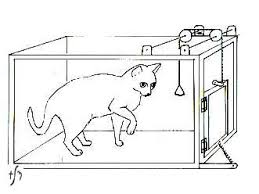
\includegraphics[scale=0.47]{slike/macka.jpg}
        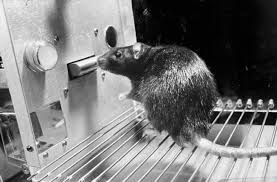
\includegraphics[scale=0.5]{slike/miska.jpg}
    \end{figure}
            
\end{frame}


\begin{frame}
    \frametitle{Okvir}
    \begin{figure}
        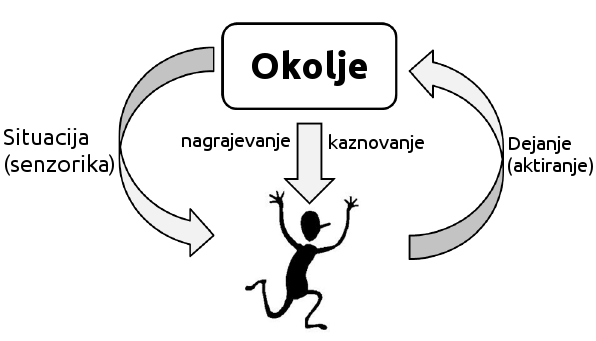
\includegraphics[scale=0.5]{slike/RLloop.png}
    \end{figure}
\end{frame}


\begin{frame}
    \frametitle{Primer 1: robot se uči hoje}
    \begin{itemize}
        \item \textbf{Situacija/Stanje}: položaj v sobi in stanje nog,
        \item \textbf{Nagrada}: $1$ za doseg vrat, $2$ za ključ, $-0.5$ za časovni korak,
        \item \textbf{Okolje}: soba in senzorji, ki govorijo o položaju,
        \item \textbf{Akcija}: Premik noge.
    \end{itemize}
\end{frame}


\begin{frame}[fragile]
    \frametitle{Primer 2: križci in krožci}
    \begin{columns}[T] % align columns
    \begin{column}{.48\textwidth}
    
    \begin{itemize}
        \item \textbf{Situacija/Stanje}: stanje na plošči,
        \item \textbf{Nagrada}: $1$ za zmago, $-1$ za poraz, $x$ za izenačenje/korak,
        \item \textbf{Okolje}: nasprotnik, plošča, sodnik, nagrajevalec,
        \item \textbf{Akcija}: postavitev $X$ oz. $O$ na ploščo.
    \end{itemize}

    \end{column}%
    \hfill%
    \begin{column}{.48\textwidth}
    
        \begin{forest}
            TTT/.style args={#1:#2}{
              make tab/.expanded=\forestove{content},
              label={\pgfkeysvalueof{/forest/label position #1}:$#2$}
            },
            TTT*/.style={
              make tab=::/::/::,
              content/.expand once=%
              \expandafter\vphantom\expandafter{\romannumeral-`0\forestov{content}},
              draw=none,
              append after command={(\tikzlastnode.north) edge (\tikzlastnode.south)},
              for descendants={before computing xy={l*=1.2}},
            },
            th/.style=thick,
            for tree={node options=draw, inner sep=+0pt, parent anchor=south, child anchor=north}
            [o:x:o/x:x:/x:o:, TTT=r:
                [o:x:o/x:x:o/x:o:, TTT=b:
                    [o:x:o/x:x:o/x:o:x, TTT=b: x]
            ]
                [o:x:o/x:x:/x:o:o, TTT=b:
                    [o:x:o/x:x:x/x:o:o, TTT=b: 1]
            ]
            ]
        \end{forest}

    \end{column}%
    \end{columns}
    \end{frame}


    \begin{frame}
        \frametitle{Ideja}
        \begin{itemize}
            \item Agent ">pade"< v okolje. 
            \item S poskušanjem se nauči pravilnih akcij.
            \item Svoje znanje izkoristi za maksimizacijo nagrade.
        \end{itemize}
        
        hipoteza o nagradi??

    \end{frame}


\begin{frame}
    \frametitle{Formalizacija: Markovski proces odločanja 1}
    \begin{definicija}[Markovska veriga]
        Slučajni proces $(S_t)_{t=0}^T$ na končnem verjetnostnem prostoru 
        $(\Omega, \mathcal{F},  P)$ je \textbf{Markovska veriga}, če velja Markovska lastnost
        $$
        P(S_{t+1} = s_{t+1}~|~S_{t} = s_{t}, ..., S_0 = s_0) = P(S_{t+1} = s_{t+1}~|~S_{t} = s_{t})
        $$
    \end{definicija}
    \pause
    \medskip
    \begin{itemize}
        \item Prihodnost je neodvisna od preteklosti, če poznamo sedanjost
        \pause
        \item $p_{ss'} := P(S_{t+1} = s'~|~S_{t} = s) \rightarrow
                \mathcal{P} := [p_{ss'}]_{s,s'\in \mathcal{S} }$, $\mathcal{S}$ 
                je množica stanj
        \item \emph{Markovska veriga} je torej dvojica $(\mathcal{S}, \mathcal{P})$
    \end{itemize}
    
\end{frame}


\begin{frame}
    \frametitle{Formalizacija: Markovski proces odločanja 2}
    \begin{definicija}[Markovski proces nagrajevanja]
        \textbf{Markovski proces odločanja} je nabor 
        $(\mathcal{S}, \mathcal{P}, \mathcal{R}, \gamma)$, kjer je
        \begin{itemize}
            \item $\mathcal{S}$ je (končna) množica stanj
            \item $\mathcal{P}$ je prehodna matrika, kjer $p_{ss'} = P(S_{t+1} = s'~|~S_{t} = s)$
            \item $\mathcal{R}$ je nagradna funkcija $\mathcal{R}_s = E[R_{t+1}~|~S_{t} = s]$
            \item $\gamma \in [0, 1]$ je diskontni faktor
        \end{itemize}
    \end{definicija}
\end{frame}


\begin{frame}
    \frametitle{Formalizacija: Markovski proces odločanja 3}
    \begin{definicija}[Markovski proces odločanja]
        \textbf{Markovski proces odločanja} je nabor 
        $(\mathcal{S}, \mathcal{A}, \mathcal{P}, \mathcal{R}, \gamma)$, kjer je
        \begin{itemize}
            \item $\mathcal{S}$ je (končna) množica stanj
            \item $\mathcal{A}$ je (končna) množica akcij oz. dejanj
            \item $\mathcal{P}$ je prehodna matrika, kjer $p_{ss'}^a = P(S_{t+1} = s'~|~S_{t} = s,
                    \mathbf{A_t = a})$
            \item $\mathcal{R}$ je nagradna funkcija $\mathcal{R}_s^a = E[R_{t+1}~|~S_{t} = s, 
                    \mathbf{A_t = a}]$
            \item $\gamma \in [0, 1]$ je diskontni faktor
        \end{itemize}
    \end{definicija}
\end{frame}


\begin{frame}
    \frametitle{Primer: MDP}
\end{frame}


\begin{frame}
    \frametitle{Agent 1}
    \begin{itemize}
        \item Strategija (angl. \textit{Policy})
        \item Vrednostna funkcija (angl. \textit{Value function})
        \item (Model)
    \end{itemize}
\end{frame}


\begin{frame}
    \frametitle{Agent 2: strategija}
    \begin{definicija}
        \begin{itemize}
            \item \textbf{Deterministična strategija} stanju $s$ priredi akcijo $a$, 
                    $$
                    \pi(s) = a.
                    $$ 
            \item \textbf{Stohastična strategija} za vsako stanje $s$ pove verjetnosti vseh 
                    možnih akcij $a$, 
                    $$
                    \pi(a | s) = P(A_t = a~|~S_t = s).
                    $$
        \end{itemize}
    \end{definicija}
\end{frame}


\begin{frame}
    \frametitle{Agent 3: povračilo}
    \begin{definicija}[Povračilo]
        $$
        G_t = R_{t+1} + \gamma R_{t+2} + ... = \sum_{k=0}^\infty \gamma^k R_{t + k + 1}
        $$
    \end{definicija}
\end{frame}


\begin{frame}
    \frametitle{Agent 4: vrednostna funkcija}
    \begin{definicija}[Vrednostna funkcija]
        \begin{itemize}
            \item \textbf{Vrednostna funkcija stanja} je pričakovana vrednost povračila, če se 
                    vedemo skladno s strategijo $\pi$ 
                    $$
                    v_\pi(s) = \mathrm{E} [G_t~|~S_t = s].
                    $$
            \item \textbf{Vrednostna funkcija akcije} je podobna prejšnji, le da sprosti prvo akcijo 
                    $$
                    q_\pi(s, a) = \mathrm{E} [G_t~|~S_t = s, A_t = a].
                    $$
        \end{itemize}
    \end{definicija}
\end{frame}


\begin{frame}
    \frametitle{Primer - križci in krožci}
\end{frame}


\begin{frame}
    \frametitle{Algoritmi - dinamično programiranje}
\end{frame}


\begin{frame}
    \frametitle{Algoritmi - Monte Carlo}
\end{frame}


\begin{frame}
    \frametitle{Algoritmi - TD($0$)}
\end{frame}


\begin{frame}
    \frametitle{Algoritmi - TD($\lambda$)}
\end{frame}


\begin{frame}
    \frametitle{Primer - kje se zatakne?}
    \begin{itemize}
        \item velike plošče
        \item pri zgornjih algoritmih hranimo vse v tabeli
    \end{itemize}
\end{frame}


\begin{frame}
    \frametitle{Nevronske mreže}
\end{frame}


\begin{frame}
    \frametitle{Motivacija - namizne igre}
    \begin{itemize}
        \item Abstraktno mišljenje.
        \item Model življenja.
        \item Testiranje algoritmov.
    \end{itemize}
\end{frame}


\begin{frame}
    \frametitle{Namizne igre - postanja}
\end{frame}


\begin{frame}
    \frametitle{Namizne igre - trening}
\end{frame}


\begin{frame}
    \frametitle{Namizne igre - tradicionalne metode}
\end{frame}


\begin{frame}
    \frametitle{Namizne igre - združevanje}
\end{frame}


\begin{frame}
    \frametitle{Nekaj rezultatov}
\end{frame}


\begin{frame}
    \frametitle{Literatura}
    \begin{thebibliography}{9}
        \bibitem{RLintro} 
        Richard S. Sutton and Andrew G. Barto. 
    \textit{Reinforcement Learning: An introduction}.
    The MIT Press, 
    2015.

    \medskip
    \medskip

    \bibitem{RLboard}
    Imran Ghory.
    \textit{Reinforcement learning in board games}.
    2004.

    \end{thebibliography}
\end{frame}


\end{document}
